
% Describe the features your language provides and explain why this set of
% features is appropriate.
\begin{frame} \frametitle{Language Features}
\begin{itemize}
\item Can declaratively enumerate 
  \begin{itemize}
  \item Cards    - name, type, effects, cost
  \item Rulesets - e.g. how many cards you draw per turn
  \end{itemize}
\item Can define complex card effects directly from Haskell
\end{itemize}
\end{frame}

{
  \setbeamercolor{background canvas}{bg=}
  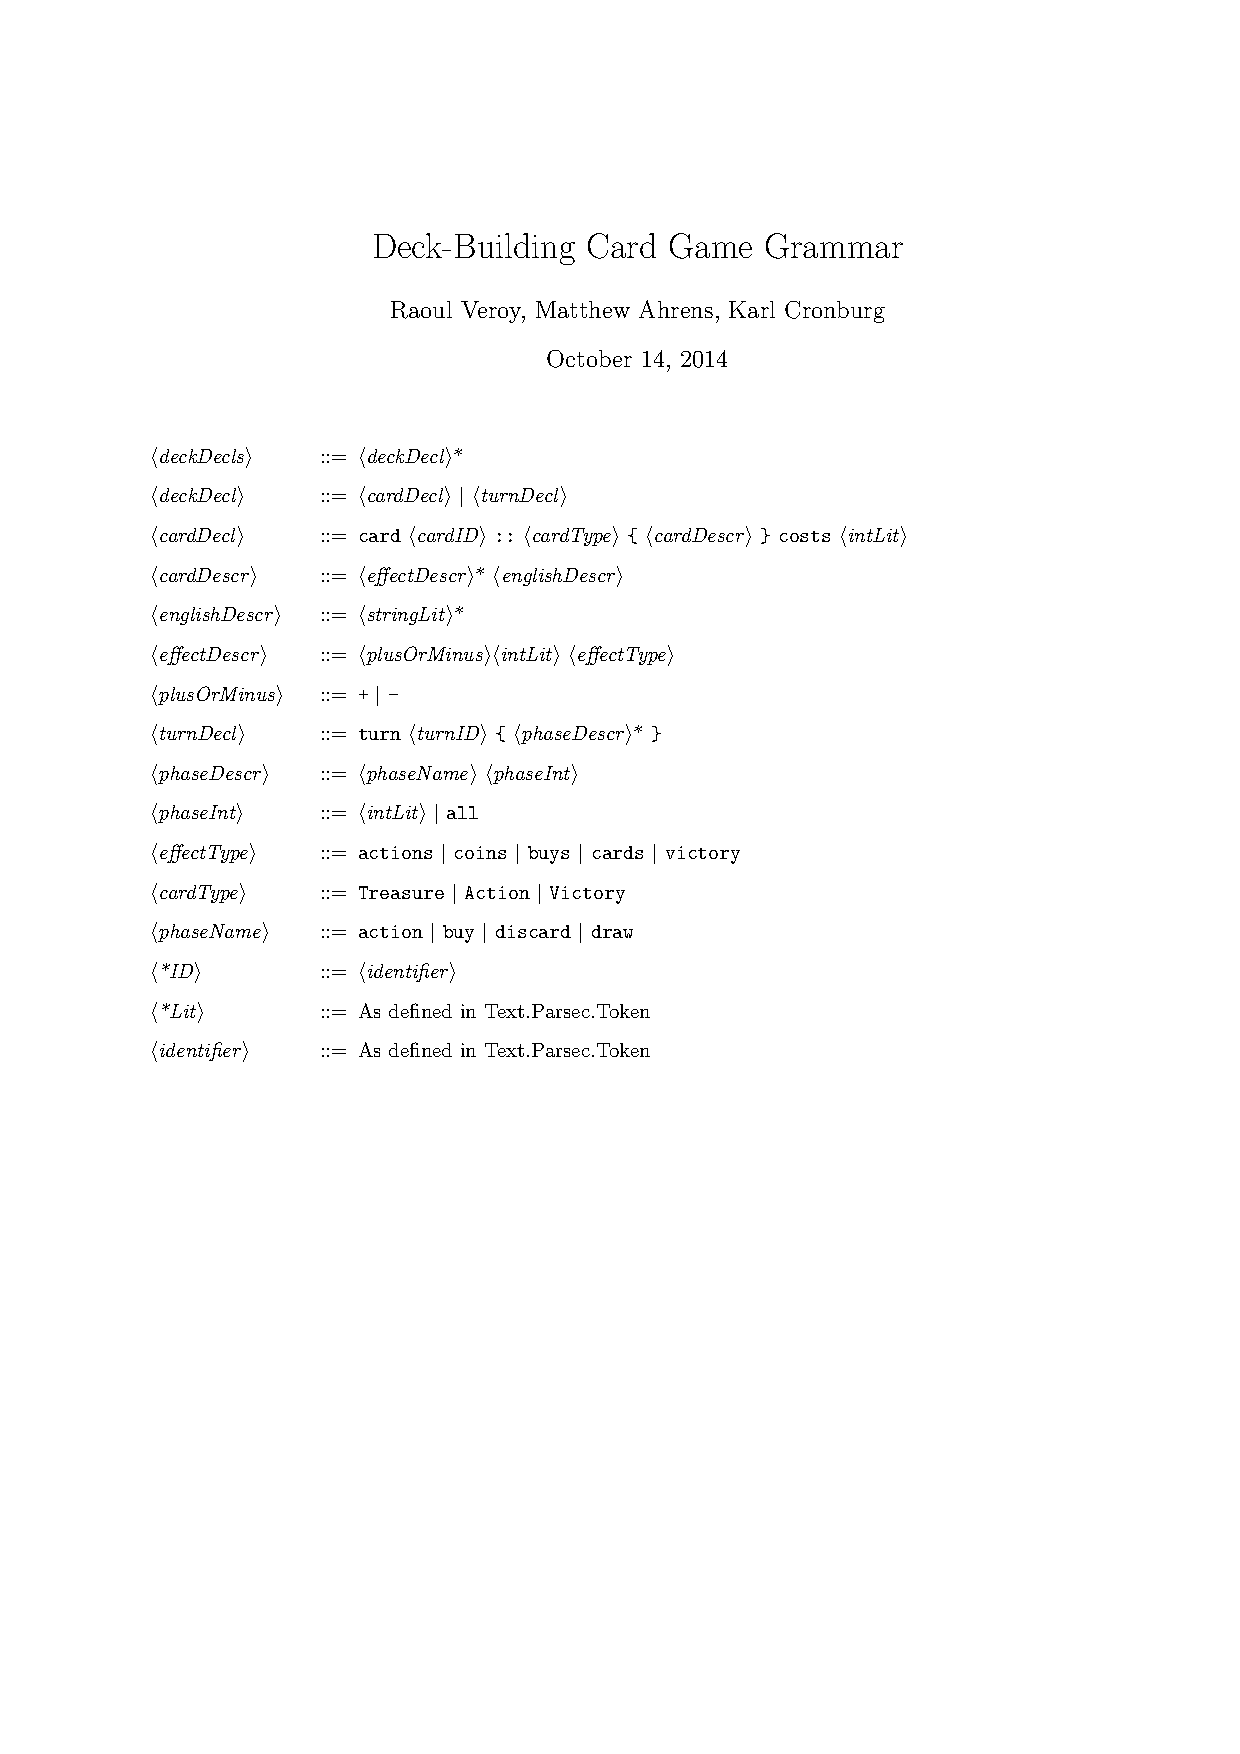
\includepdf[pages=-]{../grammar/grammar.pdf}
}
%\begin{frame} \frametitle{Language Features - Grammar}
%\begin{grammar}
%% -----------------------------------------------------------------------------
% - Top-level decls:

<deckDecls>  ::= <deckDecl>*

<deckDecl>   ::= <cardDecl> | <turnDecl>

% -----------------------------------------------------------------------------
% - Card declaration grammar rules:

<cardDecl>    ::= "card" <cardID> "::" <cardType> "{" <cardDescr> "}" "costs" <intLit>

<cardDescr>   ::= <effectDescr>* <englishDescr>

<englishDescr> ::= <stringLit>*

<effectDescr>  ::= <plusOrMinus><intLit> <effectType>

<plusOrMinus> ::= "+" | "-" 

% -----------------------------------------------------------------------------
% - Phase / rulebook declaration grammar rules:
% -   TODO: custom named phases (future), rulebook for custom rules other than turns

<turnDecl>   ::= "turn" <turnID> "{" <phaseDescr>* "}" 

<phaseDescr> ::= <phaseName> <phaseInt>

<phaseInt>   ::= <intLit> | "all"

% looks like: phases {Action 1 Buy 1 Discard all Draw 5} for standard rules.

% -----------------------------------------------------------------------------
% - Keyword and built-in-to-parsec grammar rules:
<effectType>  ::= "actions"   | "coins"  | "buys" | "cards" | "victory"

<cardType>    ::= "Treasure" | "Action" | "Victory"

<phaseName>   ::= "action"   | "buy"    | "discard" | "draw"

<*ID>         ::= <identifier>

<*Lit>      ::= As defined in Text.Parsec.Token

<identifier>  ::= As defined in Text.Parsec.Token

% Note that we don't actually need to specify the type as that is implied by the
% action
% Maybe add these back? Not sure if we need these. - Raoul
%
% <charLit>    ::= As defined in Text.Parsec.Token
%
% <stringLit>  ::= As defined in Text.Parsec.Token
%
% <identifier> ::= As defined in Text.Parsec.Token
%
% <whiteSpace> ::= As defined in Text.Parsec.Token

%\end{grammar}
%\end{frame}

% Show at least one sample program in your language and explain what it does.
\begin{frame}[fragile=singleslide] \frametitle{Example Program - Input}
\begin{columns}
  % FIRST COLUMN:
  \column{.5\linewidth}
    \begin{minted}
    [ frame=lines
    , framesep=2mm
    , fontsize=\tiny
%    , linenos
    ] {haskell}
[deck|
card Cellar  :: Action {
  +1 actions
  "Discard any number of cards."
  " +1 Card per card discarded"
} costs 2

card Chapel  :: Action {
  "Trash up to 4 cards from your hand"
} costs 2

card Village :: Action {
  +1 cards
  +2 actions
} costs 3

card Woodcutter :: Action {
  +1 buys
  +2 coins
} costs 3

card Copper :: Treasure {
  +1 coins
} costs 0

card Silver :: Treasure {
  +2 coins
} costs 3
    \end{minted}

  % SECOND COLUMN:
  \column{.5\linewidth}
    \begin{minted}
    [ frame=lines
    , framesep=2mm
    , fontsize=\tiny
%    , linenos
    ] {haskell}
card Gold :: Treasure {
  +3 coins
} costs 6

card Estate :: Victory {
  +1 victory
} costs 2

card Duchy :: Victory {
  +3 victory
} costs 5

card Province :: Victory {
  +6 victory
} costs 8

turn Dominion_Standard {
  action 1
  buy 1
  discard all
  draw 5
}





|]
    \end{minted}
\end{columns}
\end{frame}

\begin{frame}[fragile=singleslide] \frametitle{Example Program - Quasiquoter \& Code Generator}

\inputminted
[ frame=lines
, framesep=2mm
, fontsize=\fontsize{1mm}{1mm} %\tiny
, linenos
] {haskell}{CodeGen.hs}

\end{frame}

\begin{frame} \frametitle{Example Program - CodeGen Output}
\inputminted
[ frame=lines
, framesep=2mm
, fontsize=\fontsize{1mm}{1mm} %\tiny
, linenos
] {haskell}{QuoteOutput.hs}
\end{frame}

\begin{frame}[fragile=singleslide] \frametitle{Example Program - Complex Card Effects}
\begin{columns}
  \column{.5\linewidth}
    \begin{itemize}
    \item Can reference quasiquoted EDSL code from Haskell
    \item Future: design imperative-friendly (non-Haskell) EDSL for specifying
          complex card effects
    \item Example below - implementation of \verb|CELLAR| effects
    \end{itemize}
  \column{.5\linewidth} \begin{center} 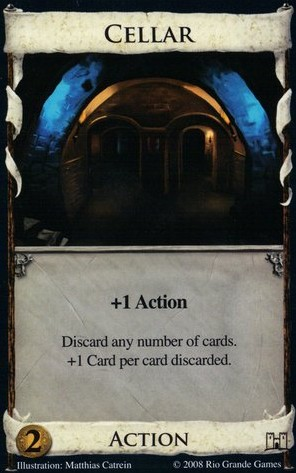
\includegraphics[width=.4\columnwidth]{cellar.jpg} \end{center}
\end{columns}
\inputminted
[ frame=lines
, framesep=2mm
, fontsize=\fontsize{1mm}{1mm} %\tiny
, linenos
] {haskell}{ComplexEffects.hs}
\footnotetext[1]{\tiny card image \& content by D. X. Vaccarino}
\end{frame}

